\documentclass[]{report}[12 pt]
\usepackage{geometry}
\usepackage{amsmath}
\usepackage{graphicx}
\usepackage{hyperref}
\geometry{margin= 1.5 cm}
\begin{document}
	\begin{titlepage}
	\begin{center}
		\vspace*{1cm}
		
		\Huge
		\textbf{Laboratory Report}
		
		\vspace{0.5cm}
		\LARGE
		X Ray Diffraction\\
		\vspace{0.5cm}
		\textbf{Guide: Prof. Sangita Bose}
		
		\vspace{1.5cm}
		
		\textbf{A R Bathri Narayanan}\\
		Roll no: P0211501\\
		UM DAE Centre for Excellence in Basic Sciences
		
		\vspace{3 cm}
		
		Report presented for the\\
		Advanced Physics Laboratory Course (PL 701)
		
		\vspace{0.8cm}
		
		
\includegraphics[width=0.4\textwidth]{cebs.jpg}
		
		\Large
		School of Physical Sciences\\
		UM-DAE Centre for Excellence in Basic Sciences\\
		Mumbai, MH, India\\
		\today
		
	\end{center}
\end{titlepage}
	\tableofcontents
\chapter{Introduction to the experiment}
	\section*{Objectives:}
\begin{enumerate}
	\item To study the generation of plasma, here using breakdown voltage method
	\item To study the Paschen curve for various gases ($N_2$ and Ar) and find its properties
	\item To try computing the value of the second Townsend coefficient $\gamma$
	\item To analyse the Plasma spectrum of the two gases ($N_2$ and Ar) and try to get the electron temperature.
\end{enumerate}

\section*{Theory:}

\chapter{Study of Paschen curves}
\section{Observations:}

\subsection{Argon where the Ring is Cathode}
\begin{center}
		\begin{tabular}{|c|c|c|c|c|c|c|}
		\hline
		Base Pressure (mbar) & Pressure (mbar) & Threshold Voltage (V) & Current (mA) & Pressure & Voltage + 25 & Current (mA) \\ \hline
		0.05                 & 0.11            & 361                   & 1            & 0.1      & 385          & 3            \\ \hline
		0.038                & 0.2             & 365                   & 2            & 0.2      & 390          & 3            \\ \hline
		0.034                & 0.3             & 302                   & 1            & 0.3      & 327          & 2            \\ \hline
		0.032                & 0.41            & 335                   & 4            & 0.4      & 360          & 5            \\ \hline
		0.029                & 0.5             & 332                   & 5            & 0.5      & 357          & 6            \\ \hline
		0.029                & 0.6             & 336                   & 6            & 0.6      & 360          & 7            \\ \hline
		0.027                & 0.72            & 340                   & 8            & 0.72     & 360          & 9            \\ \hline
	\end{tabular}\\
	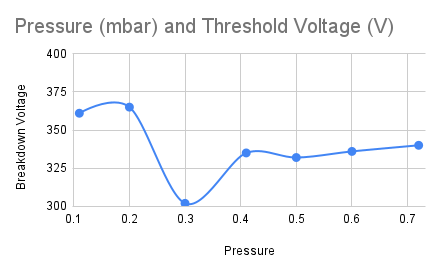
\includegraphics[width=10 cm]{plasma1.png}
\end{center}

	
\subsection{Argon when the Ring is Anode}
\begin{center}
\begin{tabular}{|c|c|c|c|c|}
	\hline
	\multicolumn{1}{|l|}{Base Pressure (mbar)} & \multicolumn{1}{l|}{Pressure (mbar)} & \multicolumn{1}{l|}{Threshold Voltage (V)} & \multicolumn{1}{l|}{Current (mA)} & \multicolumn{1}{l|}{Pressure} \\ \hline
	0.035                                      & 0.12                                 & 322                                        & 31                                & 0.1                           \\ \hline
	0.028                                      & 0.2                                  & 300                                        & 26                                & 0.2                           \\ \hline
	0.027                                      & 0.3                                  & 275                                        & 11                                & 0.3                           \\ \hline
	0.027                                      & 0.41                                 & 265                                        & 8                                 & 0.4                           \\ \hline
	0.027                                      & 0.5                                  & 264                                        & 8                                 & 0.5                           \\ \hline
	0.027                                      & 0.6                                  & 268                                        & 10                                & 0.6                           \\ \hline
	0.026                                      & 0.71                                 & 272                                        & 12                                & 0.72                          \\ \hline
\end{tabular}
	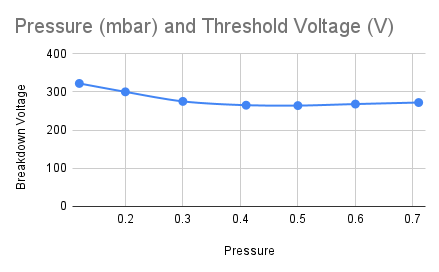
\includegraphics[width=10 cm]{plasma2.png}
\end{center}
\textit{ We are not increasing the Voltage by 25 V and analysing this time considering high current, which may damage the apparatus}
	
\subsection{Nitrogen where the Ring is Cathode}
\begin{center}
	\begin{tabular}{|c|c|c|c|c|c|c|}
		\hline
		Base Pressure (mbar) & Pressure (mbar) & Threshold Voltage (V) & Current (mA) & Pressure & Voltage + 25 & Current (mA) \\ \hline
		0.036                & 0.12            & 555                   & 3            & 0.1      & 570          & 3            \\ \hline
		0.029                & 0.2             & 525                   & 4            & 0.2      & 540          & 3            \\ \hline
		0.02                 & 0.3             & 498                   & 4            & 0.3      & 513          & 4            \\ \hline
		0.029                & 0.4             & 477                   & 5            & 0.4      & 495          & 5            \\ \hline
		0.029                & 0.5             & 478                   & 6            & 0.51     & 493          & 6            \\ \hline
		0.028                & 0.61            & 472                   & 6            & 0.61     & 487          & 7            \\ \hline
		0.029                & 0.71            & 476                   & 7            & 0.72     & 491          & 7            \\ \hline
	\end{tabular}
	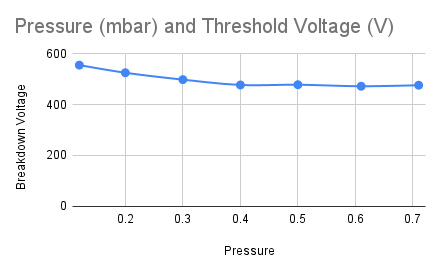
\includegraphics[width=10 cm]{plasma3.png}
\end{center}



\subsection{Nitrogen when the Ring is Anode}
\begin{center}
	\begin{tabular}{|c|c|c|c|c|}
		\hline
		Base Pressure (mbar) & Pressure (mbar) & Threshold Voltage (V) & Current (mA) & Pressure \\ \hline
		0.028                & 0.2             & 510                   & 84           & 0.2      \\ \hline
		0.03                 & 0.3             & 468                   & 71           & 0.3      \\ \hline
		0.029                & 0.4             & 394                   & 32           & 0.4      \\ \hline
		0.029                & 0.5             & 382                   & 24           & 0.51     \\ \hline
		0.029                & 0.61            & 378                   & 21           & 0.61     \\ \hline
		0.029                & 0.71            & 378                   & 18           & 0.72     \\ \hline
	\end{tabular}\\
	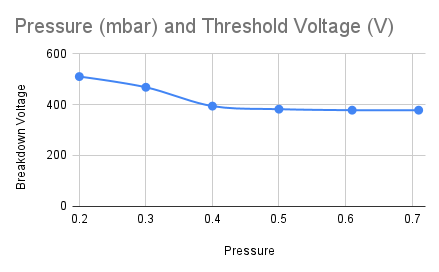
\includegraphics[width=10 cm]{plasma4.png}
\end{center}


*\textit{ We are not increasing the Voltage by 25 V and analysing this time considering high current, which may damage the apparatus}\\
The discrepancies in the shape of the Paschen curve may arise due to the fact that the Paschen curve is derived considering parallel plate condition while we have taken a ring and pipe structure.
\section{Analysis}
\subsection*{Trying to find the Townsend coefficient}
We have the Paschen curve formula
\[V = \frac{Bpd}{ln\bigg(\frac{Apd}{ln(1+\gamma^{-1})}\bigg)}\]
Minimizing, we get
\[V_{min}=2.71828\frac{B}{A}ln(\gamma^{-1}+1)\]
We have the data for B and A as (In $(Pa .m)^{-1}$)\\
\begin{center}
	\begin{tabular}{|c|c|c|}
		\hline
		Gas & A & B \\
		\hline
		$N_2$ & 13 & 413 \\
		\hline
		Ar & 16 & 240 \\
		\hline
	\end{tabular}
\end{center}
Now we make a Hypothesis to find out an approximate Townsend coefficient.\\
\textbf{Approximation:} The minimum V obtained in the experiment can be taken as the minimum V for the Paschen curve.
So if we rewrite the expression for $V_min$ as
\[\frac{1}{\gamma}=exp\bigg(\frac{V_{min}.A}{2.71828.B} \bigg)-1\]
We get approximate Townsend coefficient as
\begin{center}
	\begin{tabular}{|c|c|c|}
		\hline
		Gas & $\gamma$ when ring is anode & $\gamma$ when ring is cathode \\
		\hline
		$N_2$ & 0.07  & 0.09  \\
		\hline
		Ar & 0.06 & 0.052 \\
		\hline
	\end{tabular}
\end{center}

\chapter{Optical Emission Spectroscopy(OES)}
\section{Observations:}
\subsection{Variation of Voltage for the Same Pressure}
\subsubsection{Nitrogen}
\begin{center}
	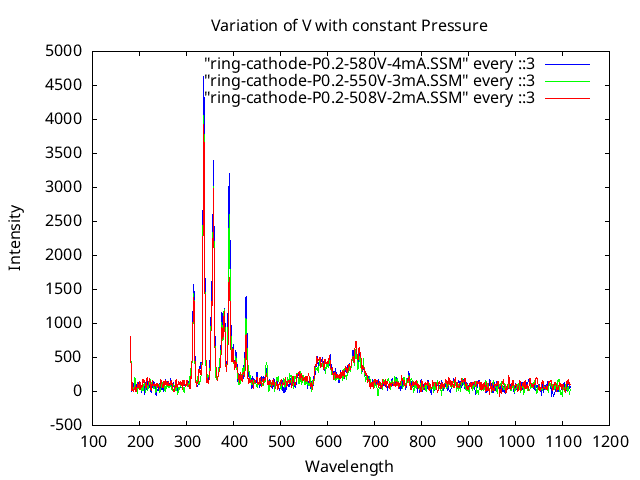
\includegraphics[width=10cm]{VvsP0.2N.png}
\end{center}
\subsubsection{Argon}
\begin{center}
	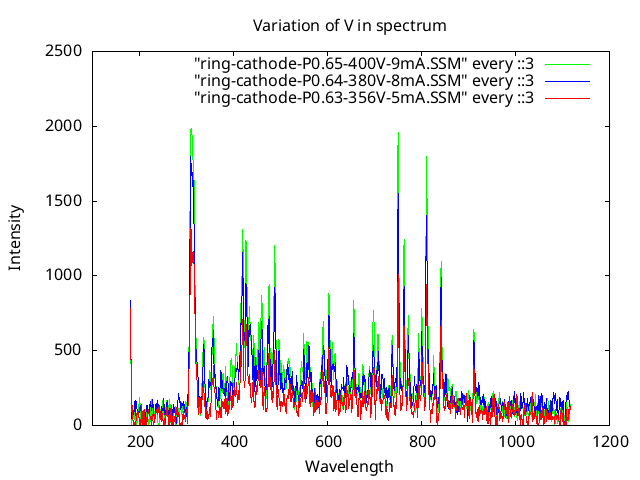
\includegraphics[width=9cm]{P0.64VAr.png}
	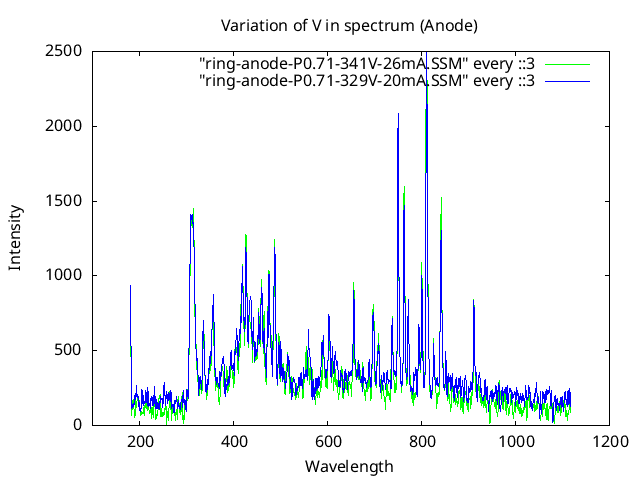
\includegraphics[width=9 cm]{P0.71V(anode)Ar.png}
\end{center}
\subsection{Variation of Pressure for the Same Voltage}
\subsubsection{Nitrogen}
\begin{center}
	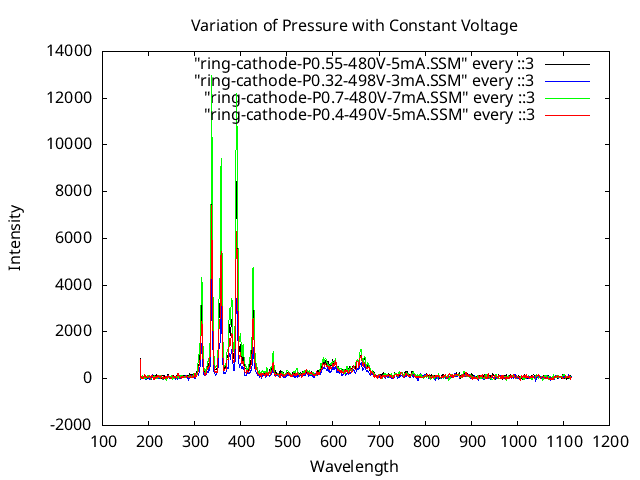
\includegraphics[width=10cm]{PvsV480N.png}
\end{center}
\subsubsection{Argon}
\begin{center}
	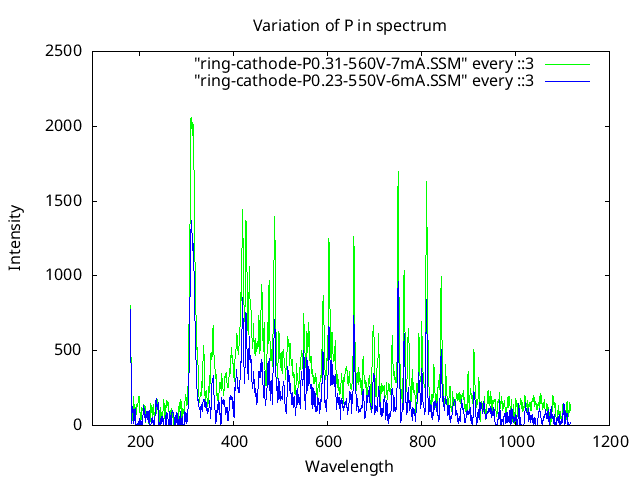
\includegraphics[width=9cm]{PV555Ar.png}
	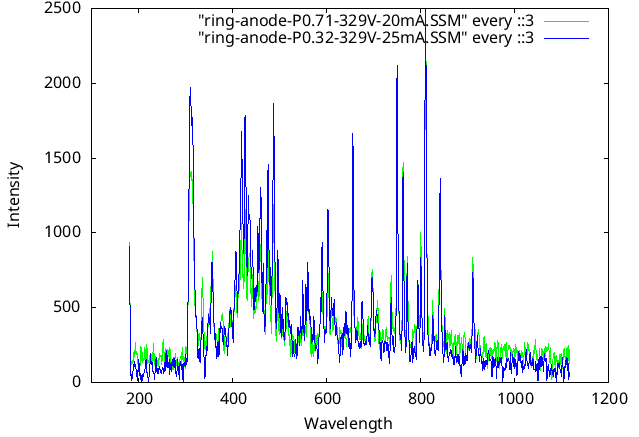
\includegraphics[width=9 cm]{PV329(anode)Armod.png}
\end{center}

\subsection{Nitrogen with ring as anode }
\begin{center}
	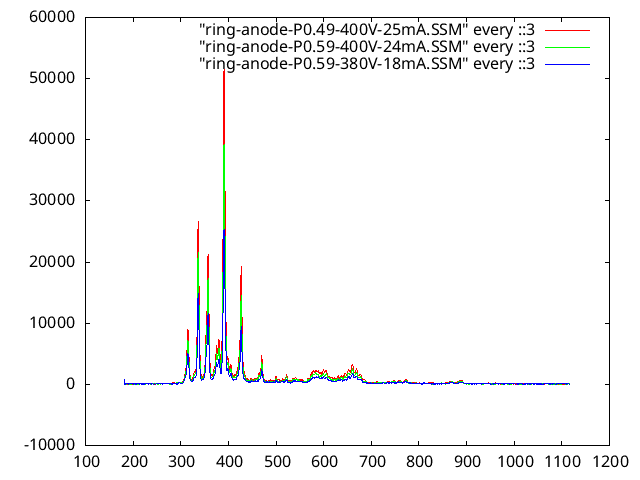
\includegraphics[width=10cm]{nitrogen_ring_anode.png}
\end{center}

\section{Analysis of the Above Graphs}
\subsubsection{Finding the electron temperature}
We find the electron temperature by using the formula
\[ln\bigg(\frac{\lambda_iI_i}{p_i}\bigg)=\frac{E_k}{kT}+C\]
We get the data
\section*{References:}
\end{document}